\documentclass{article}
\usepackage{bm}
\usepackage{graphicx}
\usepackage{amsmath}
\usepackage{enumitem}
\usepackage{xcolor}
\usepackage{float}
\usepackage{graphicx}
\usepackage{subcaption} % Required for the subfigure environment


\usepackage[a4paper, margin=1in]{geometry}

\title{Comp Project Plan}
\author{Taron Malter}
\date{September 2026}

\begin{document}

\maketitle

\section*{Introduction}

The aim of this project is to create a computational model of cell membrane potential dynamics, when interacting with each other and an embedded electrostatic field. I will adapt the model developed in the paper "Field-mediated bioelectric basis of morphogenetic prepatterning", starting with a simplified 2 cell model, and then moving to a larger network of cells aiming to see more complex behaviour and nonlinear effects of applied extracellular potentials. 

\hfill\break 
\hfill\break

\begin{flushleft}
The project has three main stages:

\begin{enumerate}

    \item Analyze and understand the behaviour of the governing differential equations of the system. And plan code structure.
    \item Write code for the Simplified 2 cell model.
    
    \begin{enumerate}[label=(\alph*)]
    
        \item Model will contain 2 cells, 6 field grid points and 1 gap junction.
        \item Analyse its behaviour and ensure everything is behaving as expected, adjust parameters if needed. 
        \item Make sure I can visualize and plot data from the model, including animations.
   
    \end{enumerate}
    
    \item Expand the model to include a larger grid with more cells and electric field grid points
     \begin{enumerate}[label=(\alph*)]
        \item Adjust equations as needed to incorparate the larger model.
        \item Make sure plotting and visualisations are working correctly, they will need adjusting
        \item Analyse behaviour of the model, by adjusting parameters and constants of the system.   \textcolor{red}{The plan needs changing somewhat since the porject has slightly changed/evolved, but I am currently here. The next thing is to redo TSE complexity for the 11x11 cell lattice and also perform other analyses that weren't possible with the 2 cell model}
        \item Incorperate stimulation of edge field points, to produce complex pattern formation after transient stimulation (either normalising or creating patterns). 
        \item Time permitting, optimise the stimulation for a specific task. 
   
    \end{enumerate}

\end{enumerate}
\begin{figure}[H]
    \centering
    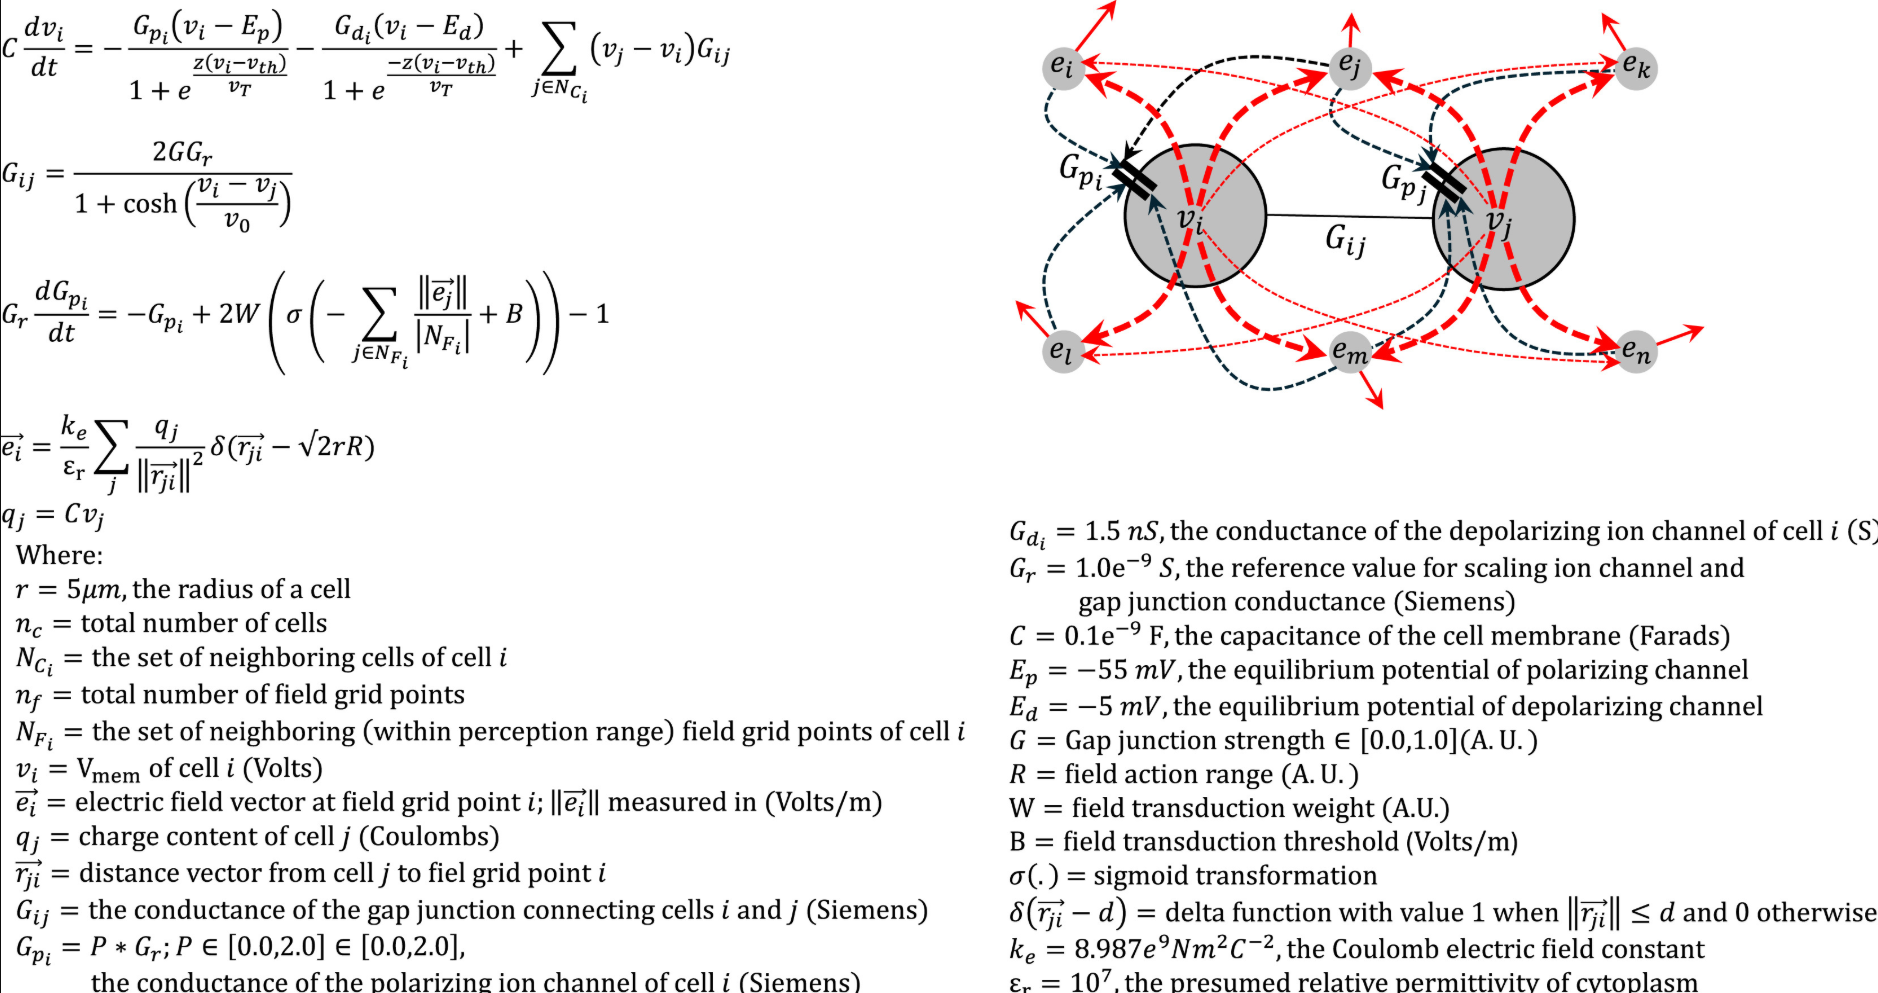
\includegraphics[width=0.6\textwidth]{Screenshot 2026-09-07 121710.png} 
    \caption{Screenshot of Computational model equations and parameters from paper}
    \label{fig:screenshot}
\end{figure}
\hfill\break 
\hfill\break

The inability for genomics to explain large scale information in biological systems, such as embryo development and body plan organisation has lead to recent research demonstrating that emergent biophysical properties of cells plays a key role in high level information in biological systems. All cells, not just neural cells have actively maintained electrical properties, the most significant of which is the membrane potential, $V_{mem}$. Cell’s $V_{mem}$ is actively maintained by a variety of ion channels, which either allow diffusion of, or actively pump electrically charged ions across the cell membrane, to maintain a specific membrane potential, which differs by tissue and cell type. Studies have shown that this membrane potential acts on two levels: at the cellular level the membrane potential is a master biophysical regulator of cell behaviour and phenotype, while on the tissue level the spatiotemporal patterns of of cell $V_{mem}$ states form an instructional code that determines global system properties such as tissue type, limb formation and homeostasis. This can even be visually seen with voltage imaging of developing frog embryos for example. And recent studies have used spatially specific artificially induced membrane potential changes to induce, eye formation, limb regeneration, and revers oncogene induced carcinogenisis.
Despite these advances, analysis of the information stored in the bioelectric networks of cells, coordinated by $V_{mem}$, the cell coupling gap junctions, and the induced electrostatic fields, is in a much earlier stage, and a complete theory of how this information is created, maintained and employed by cells to coordinate large scale behaviour has not yet been formed.
It was Burr who, observing physics progressing from particle based formulations to field theories, first proposed a bioelectric field theory for biology. And the idea of voltage gradients guiding patterning in biology. But it has taken many decades before this hypothesis has been tested and developed to a reasonable degree.

It is known that many gene expression and epigenetic targets lie downstream of changes in bioelectric state of cells. In recent studies in vivo experiments have used manipulation of membrane potentials to repair birth defects, reprogram induced tumours, and regrow normally non-regenerating frogs legs. Alongside these highly important specific discoveries, it is of great importance to have the ability to fully understand how cell membrane potentials and electric fields, coordinate pre-patterning, and allow information storage and use on the multicellular scale. Further knowledge in this field could lead to improvements in fundamental understanding of biological organisms, and future medical treatments in a wide range of fields from regeneration to oncology.

To this end we/I adapted the model in a significant recent computational paper \textbf{“Field-mediated bioelectric basis of morphogenetic prepatterning”}.
The model developed consists of a two dimensional lattice of biological cells. Each cell is equiped with a generalised polarising and depolarising ion channel, gap junctions connecting each cell to its four neighbours in the lattice, and an embedded electrostatic field, which allows a feedback mechanism between membrane potential and field excitation. Extracellular fluid and other tissue properties which would also play a role in the real world, are ignored in this model.
Here we analyse the model to understand it's information storing ability, and its characteristic behaviour.
The model has a field transduction mechanism where the ion channels (here the polarising channel), is field gated as well as voltage gated. This is implemented through the electric field vector magnitudes from the four field grid points that surround a cell being averaged, to give the sensed field by the cell. This is based on the observed electroreception phenomena in nature (refernce). Cells then radiate their electric field to the surrounding field grid points, with a distance set by the parameter termed field action range, R. 
The equilibrium potentials of the polarising and depolarising channels, Ep and Ed respectively, also play an important role in the model dynamics, which can be seen in the convergence behaviour of the governing equations. 
The model is characterised by four key parameters, that we seep over in our analysis: field waiting W, field transduction threshold B, field range R, and gap junction strength G.

\hfill\break 
\hfill\break
\section*{Analytic analysis of governing equations:} 

Conductance of gap junction connecting cells i and j: \[ G_{ij} = \frac{2GG_r}{1 + \cosh\left(\frac{v_i - v_j}{v_0}\right)} \]
The dominant behavior comes from the criticality of the cosh function: 1/cosh(x). This results in the conductivity being highest when the membrane potential of cells $i$ and $j$ are closest, and weakest when the membrane potential of cells $i$ and $j$ are furthest apart. This is because when $i$ and $j$ are similar, $\frac{1}{\cosh(0)} = 1$, and hence $G_{ij}$ is a maximum. And when $i$ and $j$ are far apart, $G_{ij}$ is minimized. Therefore, cells with initially similar membrane potentials will synchronise exponentially, while cells with strongly different $V_{mem}$ can remain seperate, they will eventually equilibriate but this happens very slowly.
\hfill\break
\hfill\break

$G_{p_i}$ \textbf{conductance of polarising ion channel of cell i:}
\[
G_r \frac{dG_{p_i}}{dt} = -G_{p_i} + 2W \left( \sigma \left( - \sum_{j \in N_{F_i}} \frac{\|\vec{e}_j\|}{|N_{F_i}|} + B \right) \right) - 1
\]

\begin{itemize}
    \item \textbf{$G_r$} is a constant, reference value for scaling ion channel gap junction conductance.
    \item \textbf{$W$} is the field transduction weight.
    \item \textbf{$\sigma$} is the sigmoid transformation.
    \item \textbf{$\bm{e}_j$} is the electric field vector at field grid point $j$.
    \item \textbf{$N_{fi}$} is the number of neighbouring grid points of cell $i$. This is a parameter which can be adjusted.
    \item \textbf{$B$} is the field transduction threshold. When the average field from the vectors, after being transformed by the weighted ($W$) sigmoid function, exceeds $B$, the \textbf{$G_p$} of the contained cell decreases, resulting in its gradual depolarization. Below the threshold, \textbf{$G_p$} increases, resulting in hyperpolarization. Thus, when \textbf{$B=0$}, all the cells depolarize, and when \textbf{$B=\infty$} the entire tissue hyperpolarizes. For intermediate values of \textbf{$B$}, heterogeneous mixtures of states can appear. This can be summarised as: Similar cells couple strongly, while different cells decouple. 
\end{itemize}

\hfill\break
\hfill\break

\textbf{Electric field vector at field grid point $i$:}
\begin{equation*}
\vec{e}_i = \frac{k_e}{\varepsilon_{\text{r}}} \sum_{j} \frac{q_j}{\|\vec{r}_{ji}\|^2} \delta(\vec{r}_{ji} - \sqrt{2}rR)
\end{equation*}

\hfill\break
\hfill\break

\textbf{Equation for $V_{mem}$ of cell $i$:}

\[
C \frac{dv_i}{dt} = - \frac{G_{p_i}(v_i - E_p)}{1 + e^{\frac{z(v_i - v_{th})}{v_T}}} - \frac{G_{d_i}(v_i - E_d)}{1 + e^{\frac{-z(v_i - v_{th})}{v_T}}} + \sum_{j \in N_{C_i}} (v_j - v_i) G_{ij}
\]

Let
\[ s(v_i)= \frac{1}{(1+e^(\frac{-z(v_i-v_{th})}{v_T)}}\]

Where $v_{th}$ is threshold voltage, and $v_t$ controls the sharpness of the transition of the sigmoid function.
With some algebra we can then write:
\[
C \frac{dv_i}{dt} = - G_{p_i}s(v_i)(v_i-E_p) - G_{d_i}[(1-s(v_i)](v_i - E_d) + \sum_{j \in N_{C_i}} (v_j - v_i) G_{ij}
\]

Now if we ignore neighboring cells then $G_{ij}=0$ (and we can drop the subscripts), and divide through by $C$. We can look at the steady state where $\frac{dv_i}{dt} =0$ and we get:
\[
0= G_{p}s(v)(v-E_p)+ G_{d}[(1-s(v)](v - E_d)
\]
Rearranging gives:
\[
v= \frac{G_{p}s(v)E_p+ G_{d}[(1-s(v)] E_d}{G_{p}s(v)+ G_{d}[(1-s(v)]}
\]

Now we can see that when $v<<v_{th}$ we have  $\frac{1}{1+e^(large)}$ so $s(v) \approx 0$. Therefore the membrane equation becomes $C\frac{dv_i}{dt} = -G_d(v-E_d)$ This has solution of the form:
\[ v(t) = E_d + [v(0)-E_d]e^{\frac{-G_dt}{C}} \]

So as $t$ progresess the voltage is driven towards $E_d =-55mV$ (voltage set from paper), with characteristic time $\tau=\frac{C}{G_d} \approx 67 ms$.
When $v>>v_{th}$ the same reasoning and working leads to the membrane voltage being driven towards $E_p = -55mV$ with a characteristic time $\tau=\frac{C}{G_p}\approx 100 ms$.

\hfill\break
\hfill\break


\section*{2 -- Cell model reproducing expected behaviour:} 
\begin{enumerate}
    \item \textbf{Effec of $B$ on behaviour:} setting $B$ from $B = 0$ up to $B = 0.01$ both cells depolarise. While setting $B = 0.03$, the cells hyperpolarise. At $B = 0.02$ the cells remain roughly at their initial states and don't equalise toward one value. For values of $W = 100, E_p = -55,  
    E_d = -5, v_i = -55.0, v_j = -5.0$
    \item \textbf{Effec of $W$ on behaviour:}  
\end{enumerate}


\begin{figure}[H] 
\centering 

% --- First Row of Subfigures ---
\begin{subfigure}[b]{0.32\textwidth} 
    \centering 
    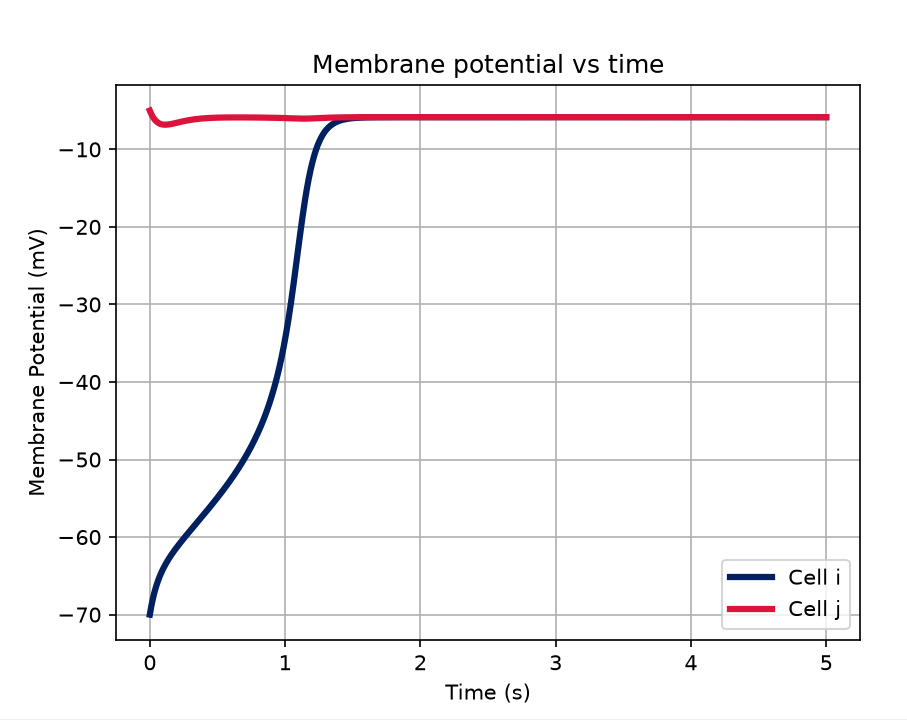
\includegraphics[width=\linewidth]{Screenshot 2026-09-20 175230} 
    \caption{Membrane potentials.} 
    \label{fig:sub-eq1} 
\end{subfigure} 
\hfill 
\begin{subfigure}[b]{0.32\textwidth} 
    \centering 
    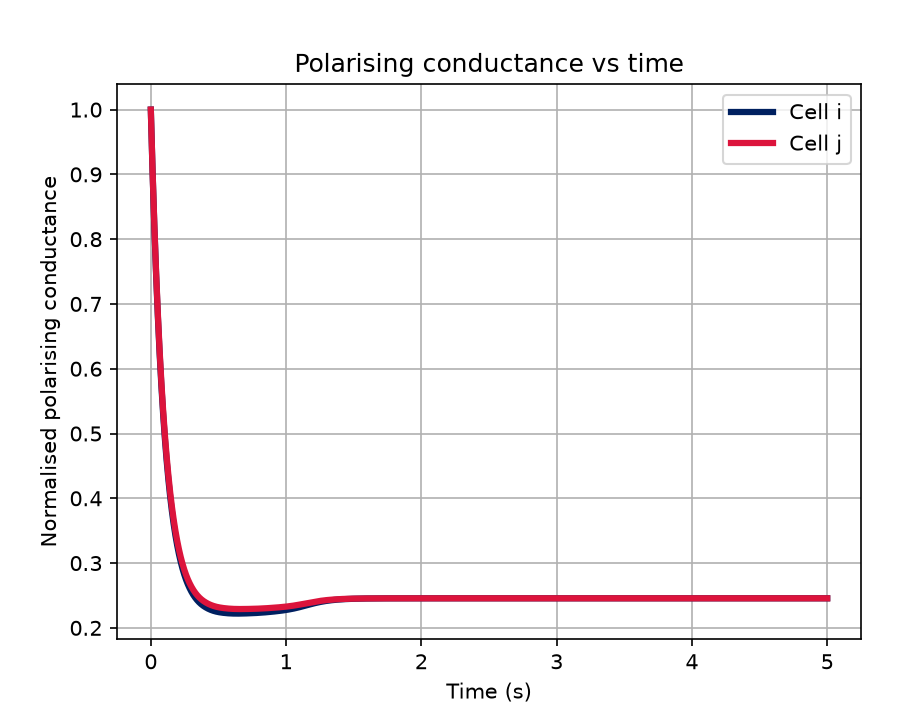
\includegraphics[width=\linewidth]{Screenshot 2026-09-20 175255} 
    \caption{Polarising channel conductance.} 
    \label{fig:sub-eq2} 
\end{subfigure} 
\hfill 
\begin{subfigure}[b]{0.32\textwidth} 
    \centering 
    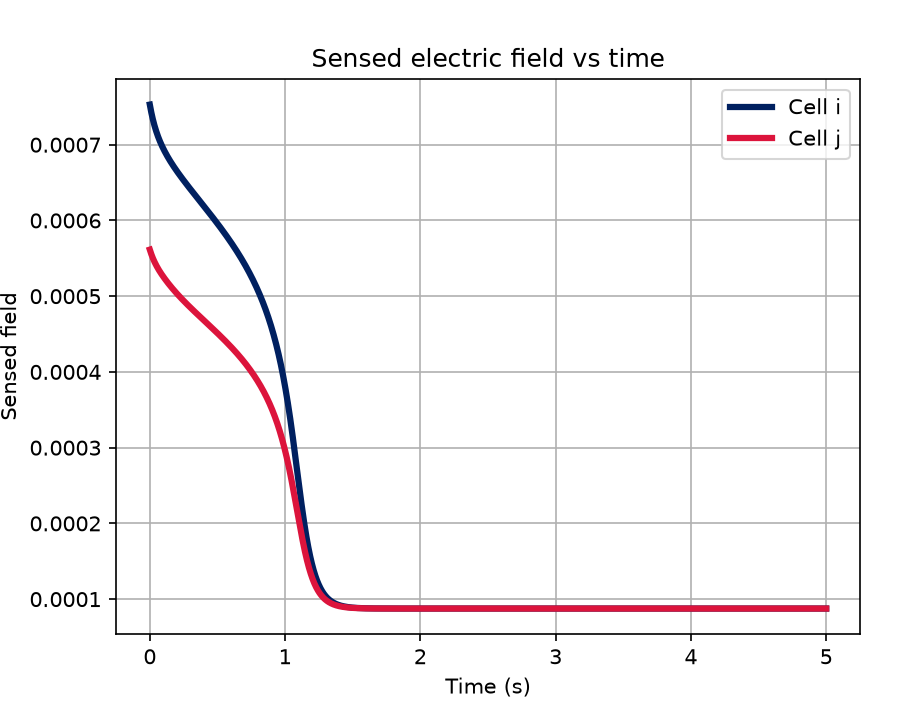
\includegraphics[width=\linewidth]{Screenshot 2026-09-20 175308} 
    \caption{Sensed electric fields.} 
    \label{fig:sub-eq3} 
\end{subfigure}

\vspace{2ex} % Adds vertical space between the two rows

% --- Second Row of Subfigures ---
\begin{subfigure}[b]{0.32\textwidth} 
    \centering 
    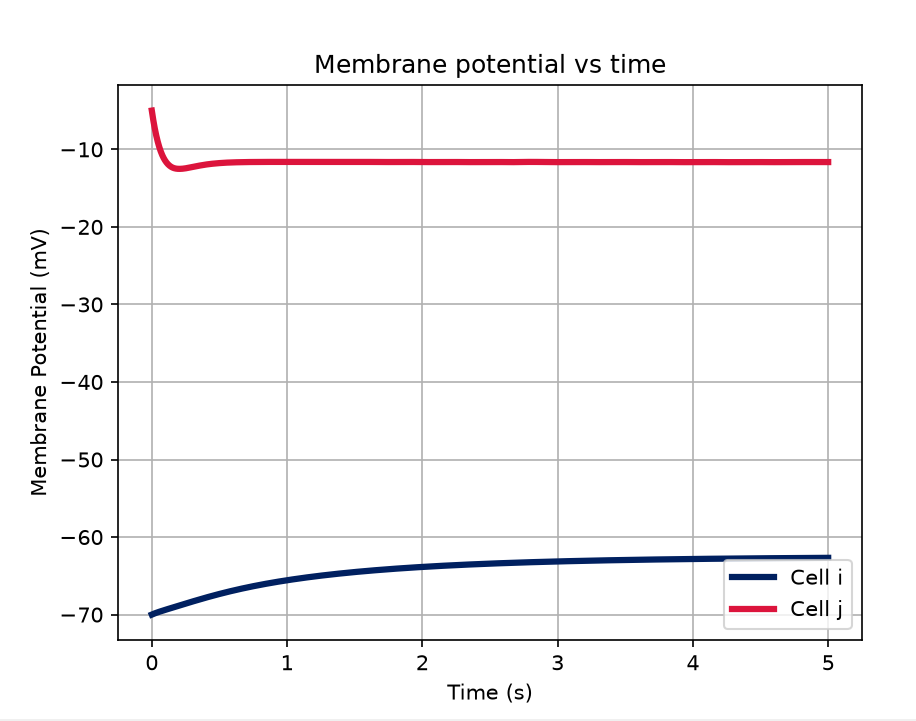
\includegraphics[width=\linewidth]{Screenshot 2026-09-20 174538} % Replace with your image path
    \caption{Membrane potentials.} 
    \label{fig:sub-eq4} 
\end{subfigure} 
\hfill 
\begin{subfigure}[b]{0.32\textwidth} 
    \centering 
    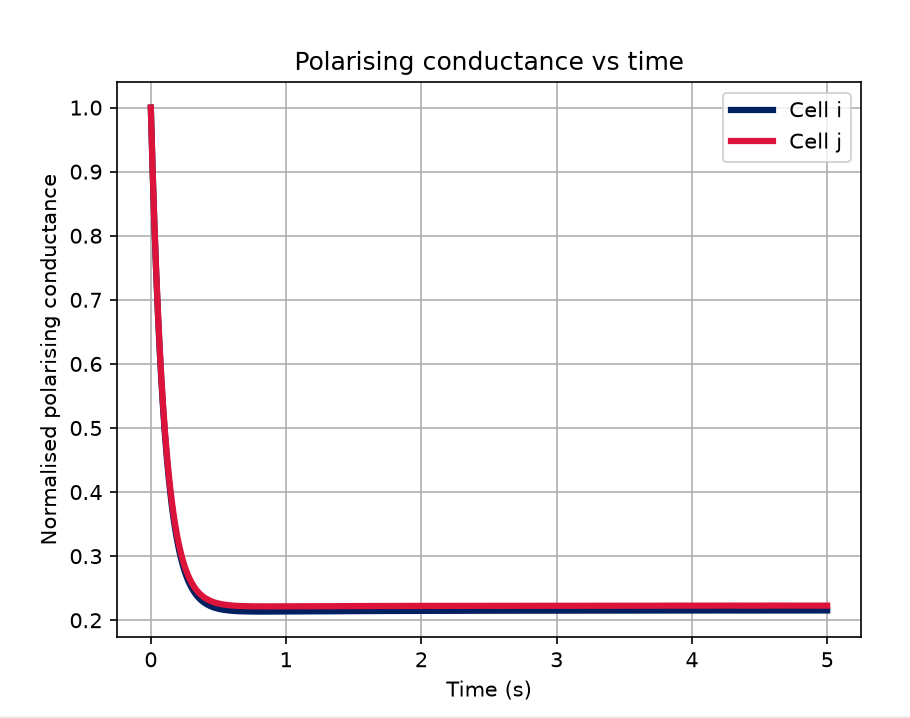
\includegraphics[width=\linewidth]{Screenshot 2026-09-20 174627} % Replace with your image path
    \caption{Polarising channel conductance.} 
    \label{fig:sub-eq5} 
\end{subfigure} 
\hfill 
\begin{subfigure}[b]{0.32\textwidth} 
    \centering 
    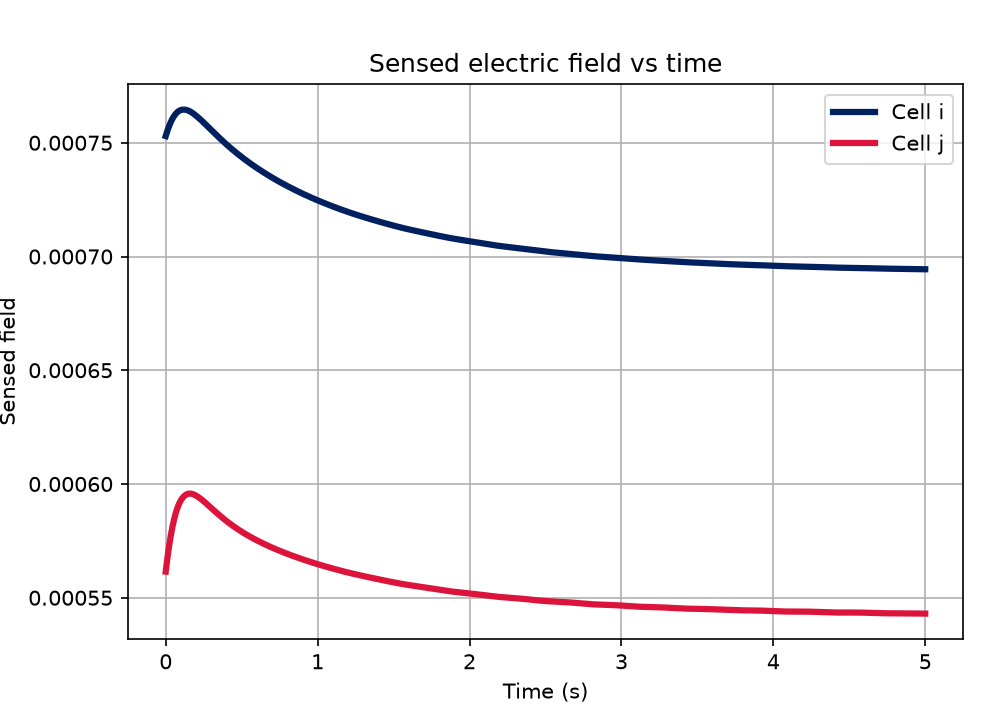
\includegraphics[width=\linewidth]{Screenshot 2026-09-20 174729} % Replace with your image path
    \caption{Sensed electric fields.} 
    \label{fig:sub-eq6} 
\end{subfigure}

% Main Overall Caption and Label 
\caption{3 main graphs showing characteristic behaviour of system's governing differential equations, for 2 cell model. (a) -- (c)  with $E_p = -55$, $E_d = -5$, $z = 3.0$, $v_{th} = -27$ and $G = 0.01$. For (d) -- (f) $E_p = -70$, $E_d = -5$, $z = 3.0$, $v_{th} = -27$ and $G = 0.01$, here graphs have separated and do not converge because, $E_p$, $G = 0.03$
$E_d$, $z = 3$ determine convergence behaviour. Complexity plot for (a) -- (c) and (d) -- (f), are Figure 3 (a) and (c) respectively \color{red}{need to properly update these graphs}.} 
\label{fig:combined_screenshots} 
\end{figure}





\begin{figure}[p] % [p] gives it a dedicated page if it's too tight for [H]
    \centering
    
    % === ROW 1 ===
    \begin{subfigure}[b]{0.45\textwidth}
        \centering
        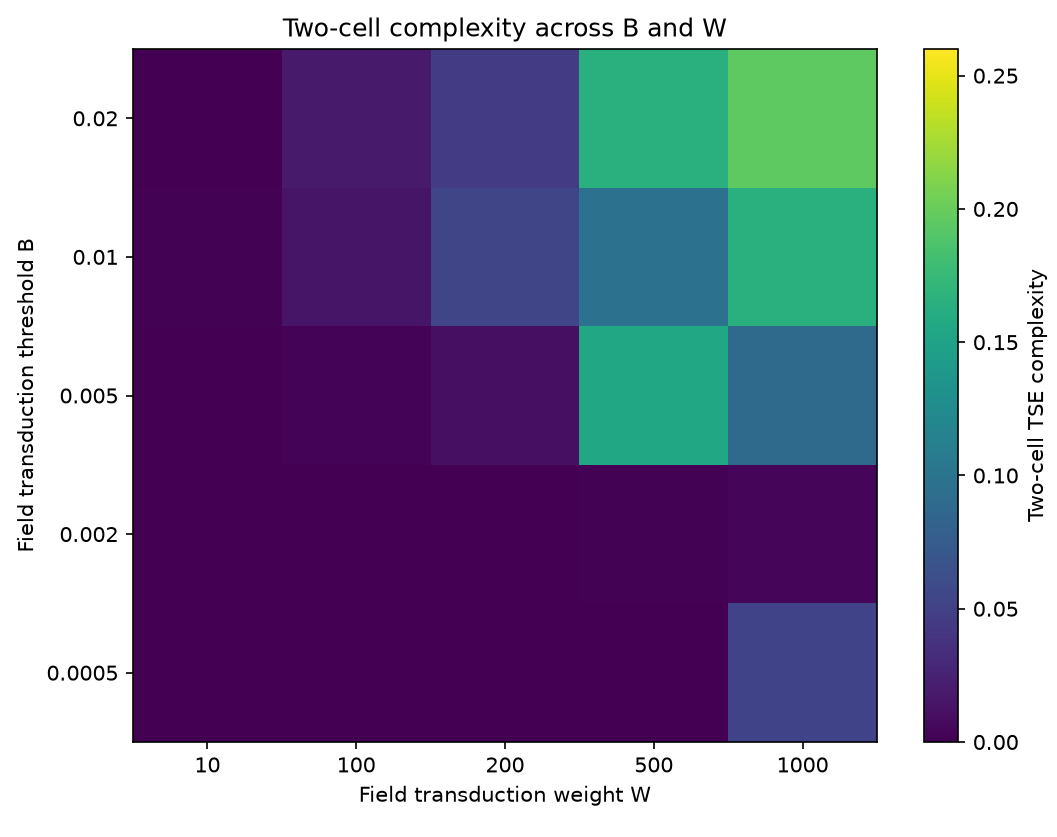
\includegraphics[width=\linewidth,height=0.17\textheight,keepaspectratio]{Screenshot 2026-10-05 135359}
        \caption{TSE heatmap for $E_p = -55$, $E_d = -5$, $v_{th} = -27$, $z = 3.0$, $G = 0.1$.}
        \label{fig:heatmap-a}
    \end{subfigure}
    \hfill
    \begin{subfigure}[b]{0.45\textwidth}
        \centering
        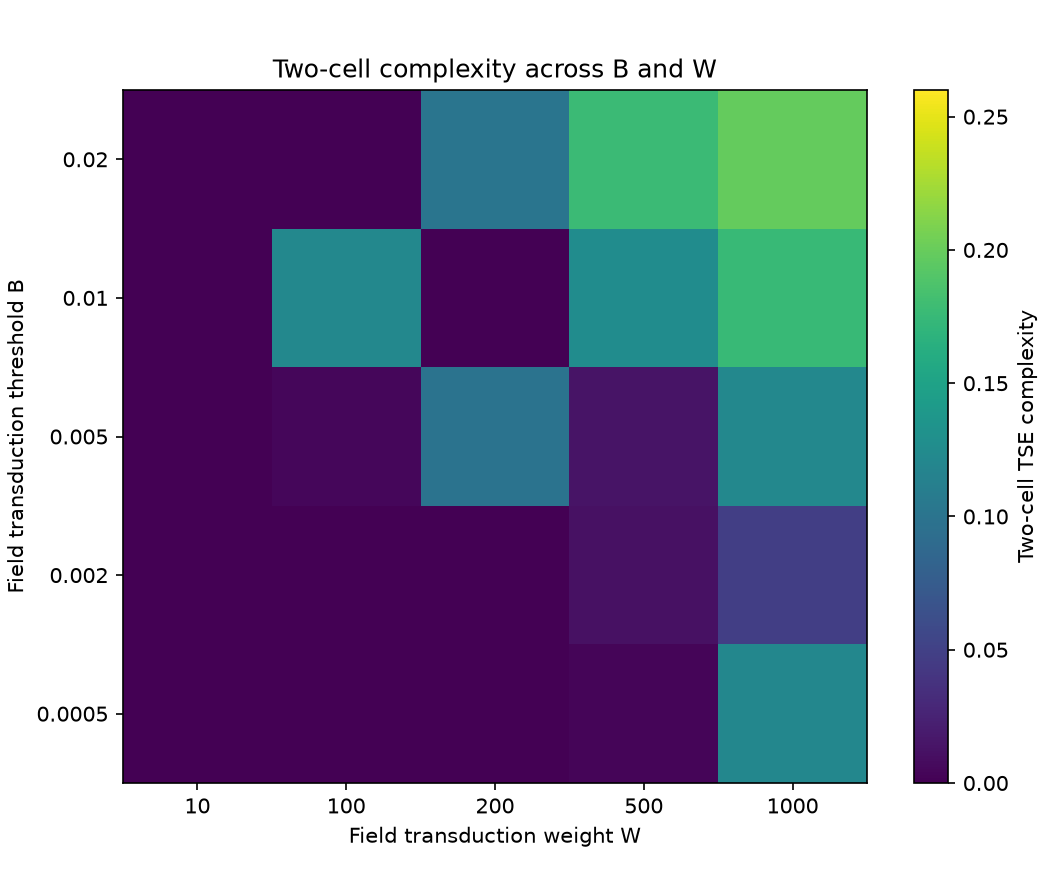
\includegraphics[width=\linewidth,height=0.17\textheight,keepaspectratio]{Screenshot 2026-10-05 135919}
        \caption{TSE heatmap for $E_p = -55$, $E_d = -15$, $v_{th} = -27$, $z = 3.0$, $G = 0.1$.}
        \label{fig:heatmap-b}
    \end{subfigure}
    
    \vspace{0.1cm}
    
    % === ROW 2 ===
    \begin{subfigure}[b]{0.45\textwidth}
        \centering
        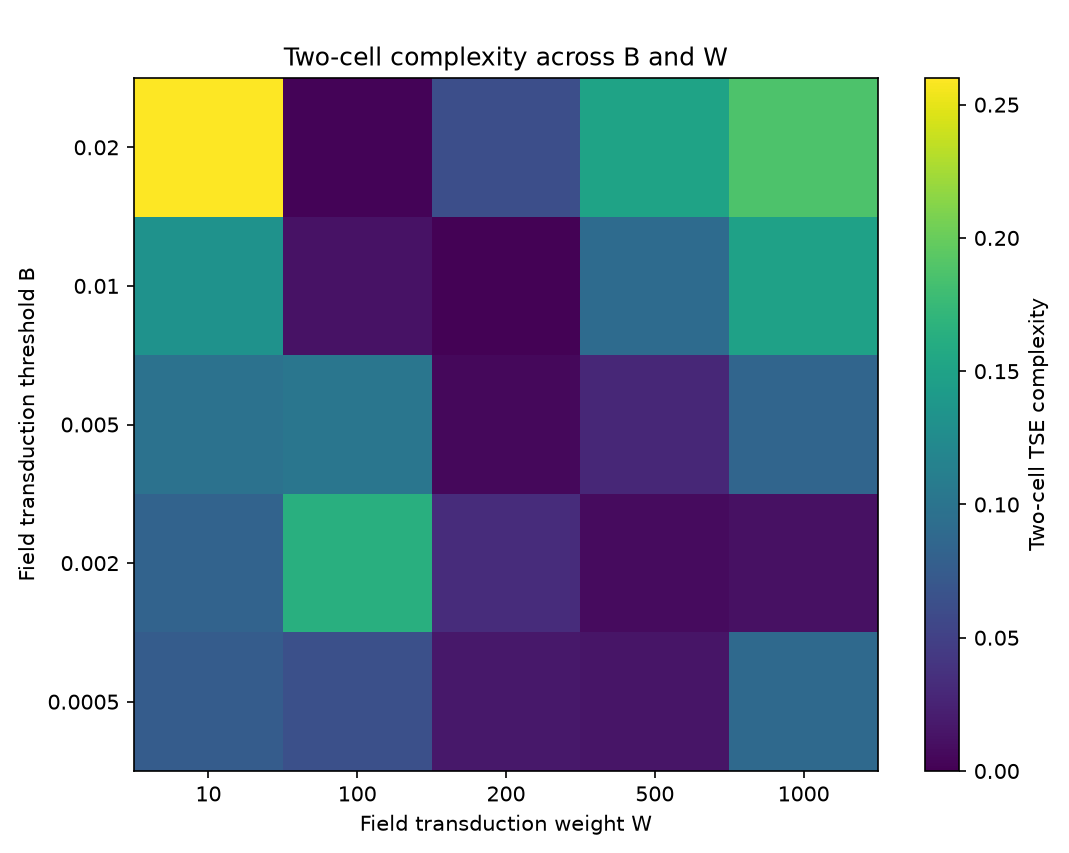
\includegraphics[width=\linewidth,height=0.17\textheight,keepaspectratio]{Screenshot 2026-10-05 140038}
        \caption{TSE heatmap for $E_p = -70$, $E_d = -5$, $v_{th} = -27$, $z = 3.0$, $G = 0.1$.}
        \label{fig:heatmap-c}
    \end{subfigure}
    \hfill
    \begin{subfigure}[b]{0.45\textwidth}
        \centering
        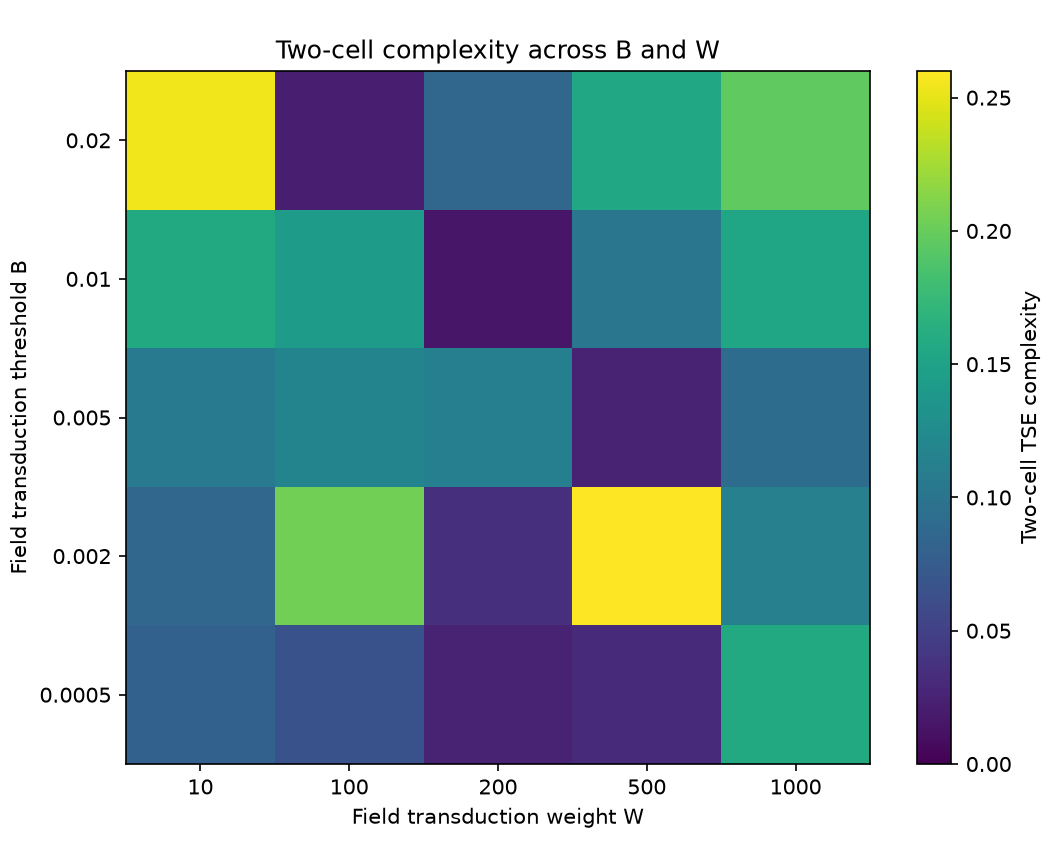
\includegraphics[width=\linewidth,height=0.17\textheight,keepaspectratio]{Screenshot 2026-10-05 140809}
        \caption{TSE heatmap for $E_p = -70$, $E_d = -15$, $v_{th} = -27$, $z = 3.0$, $G = 0.1$.}
        \label{fig:heatmap-d}
    \end{subfigure}

    \vspace{0.1cm}
    
    % === ROW 3 ===
    \begin{subfigure}[b]{0.45\textwidth}
        \centering
        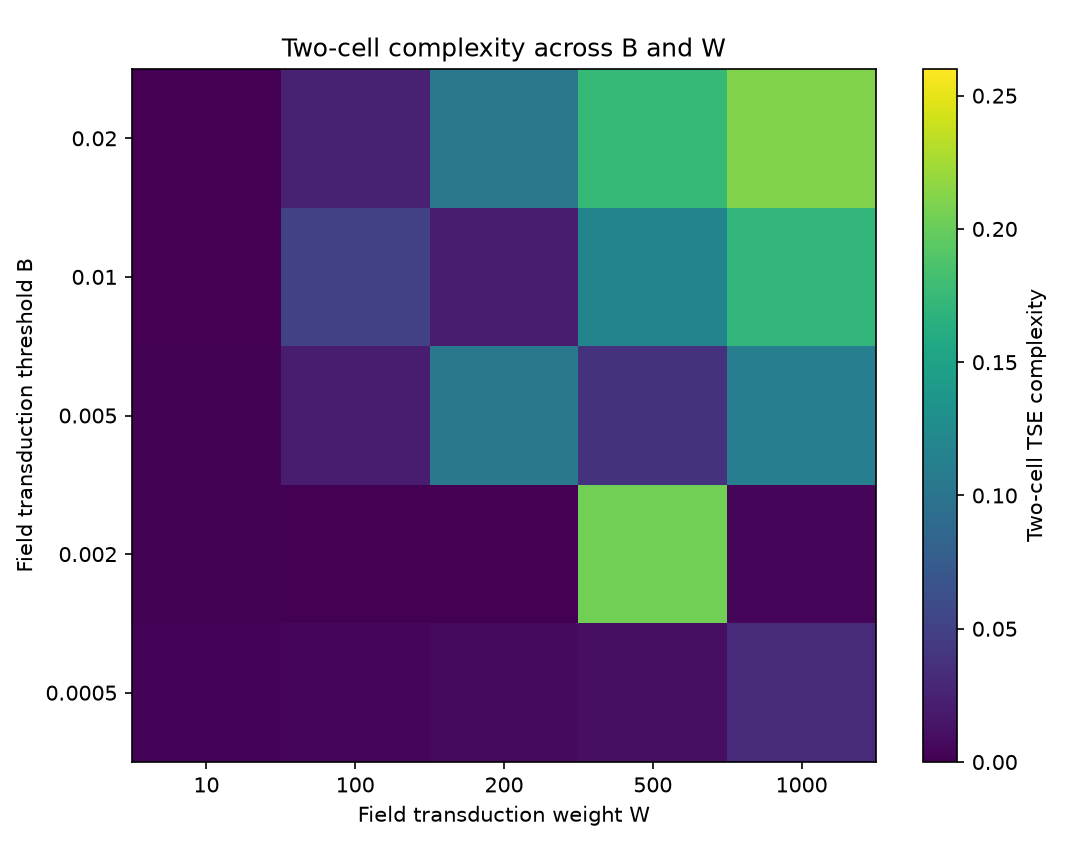
\includegraphics[width=\linewidth,height=0.17\textheight,keepaspectratio]{Screenshot 2026-10-05 141038}
        \caption{TSE heatmap for $E_p = -70$, $E_d = -15$, $v_{th} = -27$, $z = 3.0$, $G = 0.8$.}
        \label{fig:heatmap-e}
    \end{subfigure}
    \hfill
    \begin{subfigure}[b]{0.45\textwidth}
        \centering
        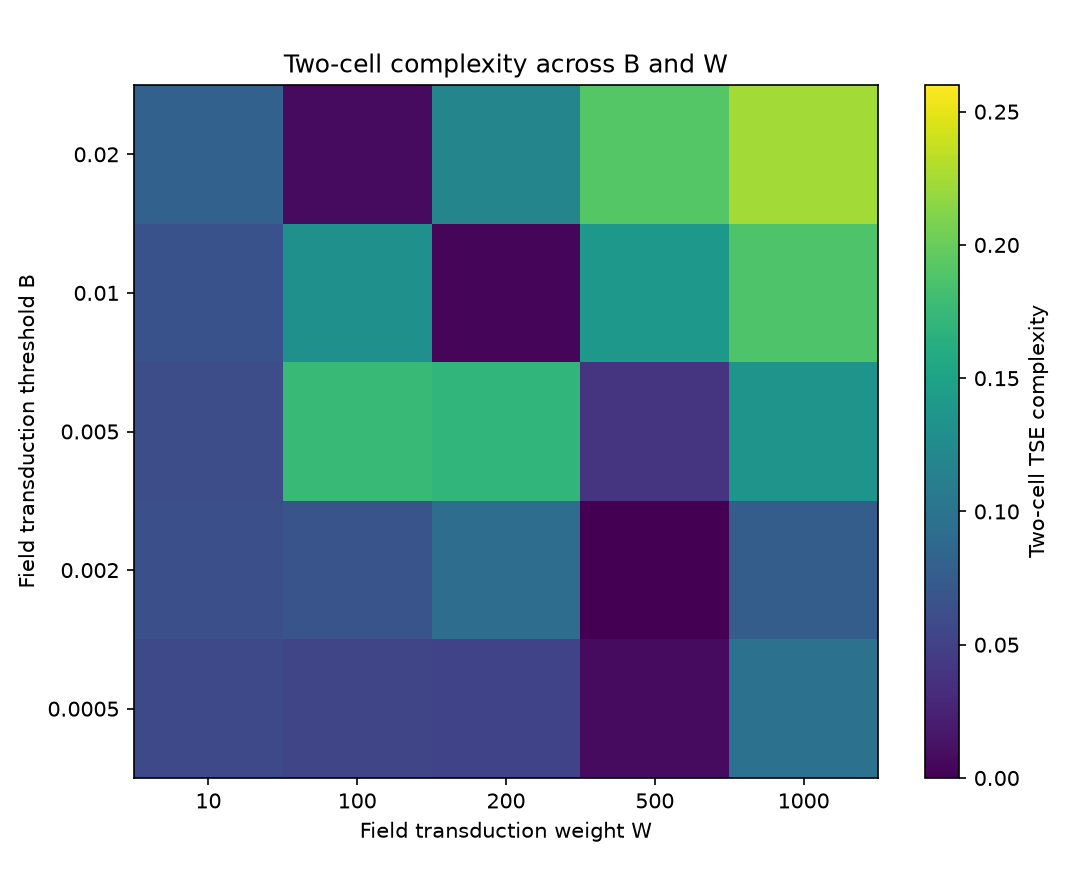
\includegraphics[width=\linewidth,height=0.17\textheight,keepaspectratio]{Screenshot 2026-10-06 141428}
        \caption{TSE heatmap for $E_p = -70$, $E_d = -15$, $v_{th} = -20$, $z = 3.0$, $G = 0.1$.}
        \label{fig:heatmap-f}
    \end{subfigure}

    \vspace{0.1cm}
    
    % === ROW 4 ===
    \begin{subfigure}[b]{0.45\textwidth}
        \centering
        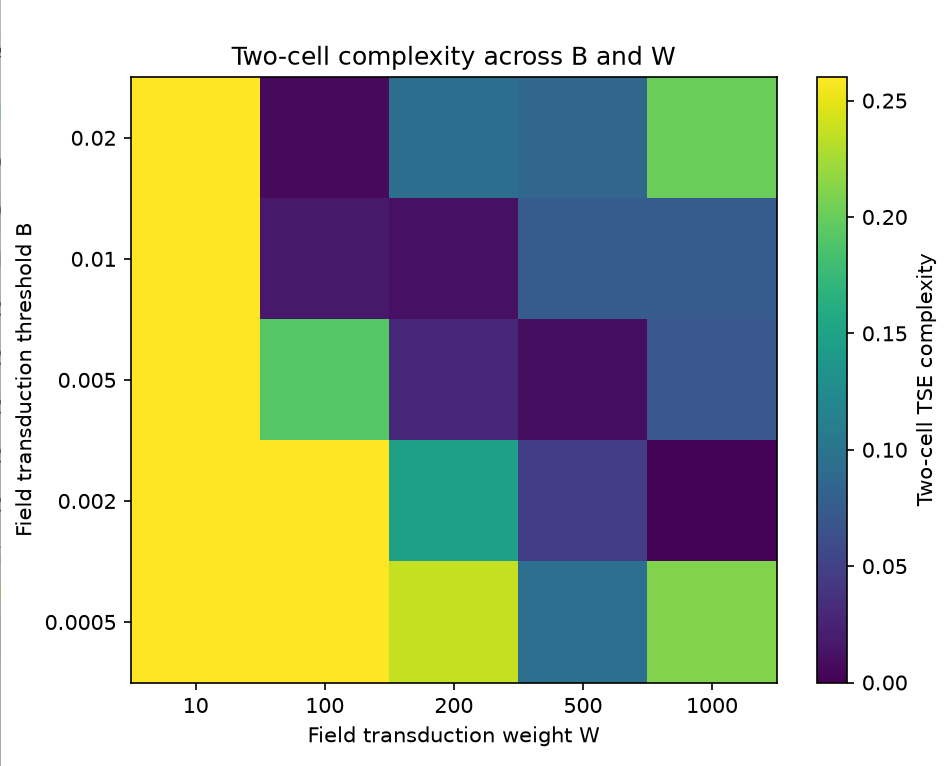
\includegraphics[width=\linewidth,height=0.17\textheight,keepaspectratio]{Screenshot 2026-10-06 142044}
        \caption{TSE heatmap for $E_p = -55$, $E_d = -5$, $v_{th} = -27$, $z = 5.0$, $G = 0.1$.}
        \label{fig:heatmap-g}
    \end{subfigure}
    \hfill
    \begin{subfigure}[b]{0.45\textwidth}
        \centering 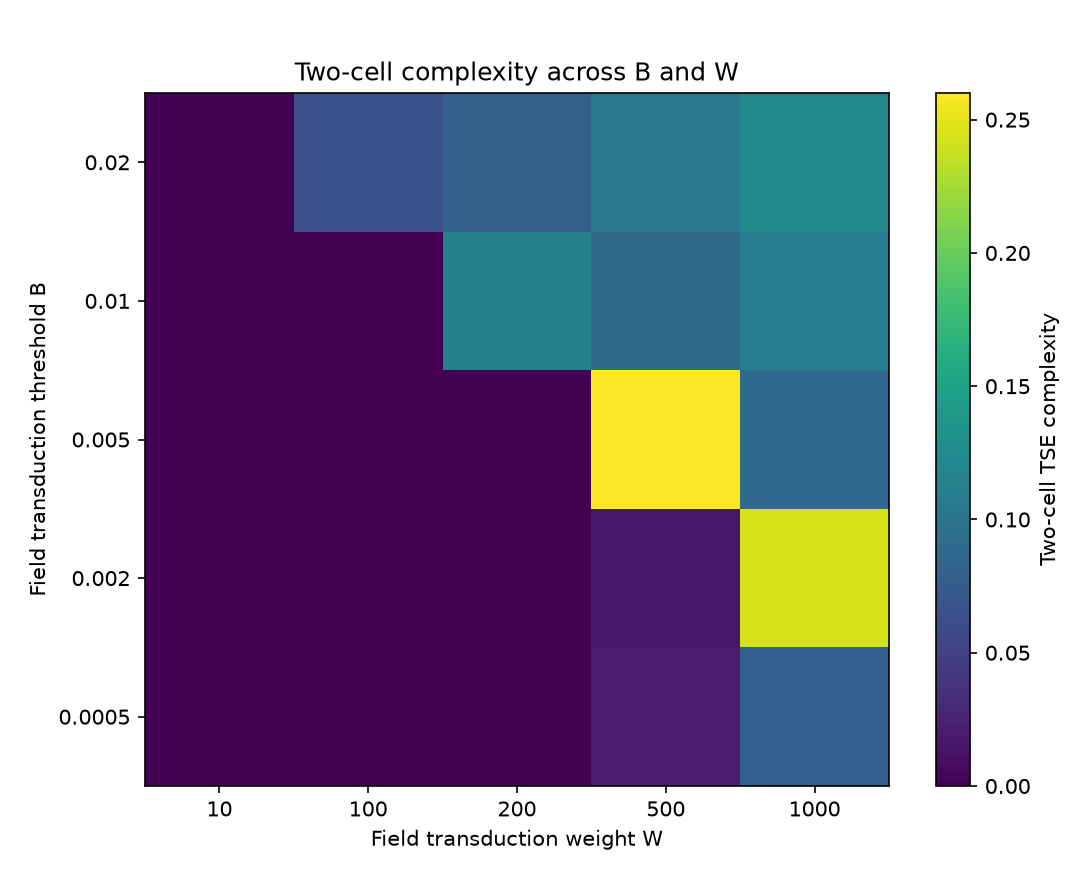
\includegraphics[width=\linewidth,height=0.17\textheight,keepaspectratio]{Screenshot 2026-10-06 142757}
        \caption{TSE heatmap for $E_p = -55$, $E_d = -5$, $v_{th} = -20$, $z = 1.0$, $G = 0.1$.}
        \label{fig:heatmap-h}
    \end{subfigure}
    
    \vspace{0.2cm}
    
    % Main Overall Caption
    \caption{2 cell TSE complexity heatmap plots, for changing values of W and B. Each plot has different $E_p$, $E_d$, $v_{th}$, $z$ and $G$ values. (a) -- (d) changing $E_p$ and $E_d$. (d) -- (f) changing $G$. (f) -- (h) changing $z$. And $(h)$ changing $v_{th}.$}
    \label{fig:all_heatmaps_grid}
\end{figure}


\end{flushleft}

\hfill\break

\begin{flushleft}
    
\textbf{Complexity analysis: 2 cell model}
\hfill\break
\hfill\break
Before expanding to a larger lattice of cells, analysis was performed on the 2 Cell model, to analyse simple behaviour and confirm analysis methods. To quantify the information in the system, Tononi-Sporns-Edelman (TSE) complexity analysis was used. TSE was developed in the context of neural systems, but here we apply it to a lattice of non-neural cells. It is a measure of how much a system contains parts that behave independently, while still being strongly integrated into a coherent whole. Here it is quantifying the compromise between integration and segregation of the $V_{mem}$ states and (when using larger lattice of cells) patterns. This means that when the model is completely integrated with the cells behaving synchronously, or when the cell's behavior is completely segregated and not effecting one another, the TSE complexity is zero. TSE is maximized when there is a balance between integration and segregation, so that the cells behave independently but still effect each other. We used TSE defined as:

$$\text{TSE}(X) = \sum_{j=1}^{n/2} \left[ \langle H(X_{k_j}) \rangle - \frac{k}{n} H(X) \right]$$

where 

$$H(X) = -\sum_{x \in X} p(x) \log p(x)$$

is the Shannon entropy. Here, \(H(X)\) is the joint entropy of the entire system of cells, while \(\langle H(X_k^j)\rangle\) is the average joint entropy of all subsets containing \(k\) cells. Here for the 2 cell model, this simplifies to 
$$TSE = \frac{1}{2}(H(X_1) + H(X_2) - H(X_1, X_2))$$
which is plotted as a function of W and B in Figure 3. Later when the number of cells is increased, we will also plot TSE as a function of the field range R, but this can't be done with the current simplified case.

\hfill\break
\hfill\break
From \textbf{Figure 3 (a) -- (c)}, it can be seen that decreasing $E_d$, and therefore decreasing the difference between $E_d$ and $E_p$, has little effect on the TSE plots, while decreasing $E_p$ increased complexity for lower values of $W$, and especially at higher values of $B$. In \textbf{(d)} decreasing $E_p$ and $E_d$ increased the complexity for lower values of $B$. Significantly increasing G from \textbf{(d)} to \textbf{(e)} concentrated the complexity in high values of $W$ and $B$, while reducing it elsewhere. Decreasing $v_{th}$ in \textbf{(f)} in relation to \textbf{(a)} increased complexity uniformly across $W$ and $B$ sweep, and visa versa. Higher values of z in \textbf{(g)} increased complexity for low $W$ and high $B$ values. In \textbf{(h)} increasing $v_{th}$ from $-27$ to $-20$ mV, significantly decreased complexity except at specific regions for high values of $W$ and lower values of $B$, creating an unusual pattern, relative to \textbf{(a)}. 

The above behavior follows the expected biophysics of the model. 
It can be seen from the analytical analysis above that $E_p$ and $E_d$ are the preffered polarised/depolarised membrane states, so changes in these alteres how easily cells can transition between states (check more this), thus altering how heterogeneous the cell behaviour can be.  
Higher W increases the strength of the field feedback, so changing parameters which effect membrane potential or field sensing will generally have a bigger effect when W is large(?).  
B shifts the field-transduction sigmoid relative to the sensed field, so changing  $E_p$ and $E_d$ which changes the voltages and therefore the fields can move the system into or out of a sensitive part of the sigmoid, and this likely explains why some effects appear at specific B values. 

Increasing gap-junction coupling $G$ pushes neighboring cells toward similar voltages, so stronger coupling therefore tends to synchronize the cells and suppress independent behavior, this can reduce complexity over much of the $W$ and $B$ parameter space. Strong field feedback which corresponds to large $W$, and an appropriate $B$, is then needed to overcome that homogenizing effect, which explains why complexity becomes concentrated in a smaller high $W$ and $B$ region. \textbf{This makes sense and seems to be relatively independent of other parameters}.

Larger $z$ makes the voltage dependence steeper. So cells behave more like switches around $V_{th}$, strengthening the distinction between polarized and depolarized states. This can support more pronounced spatial patterns and hence higher complexity. However strong field weighting $W$ and high threshold $B$ likely combine to reduce this effect, which explians \textbf{Figure 3 (g)}. The Small $z$ makes the response smoother and weakens this bistability, so it is understandable that complexity only survives in a narrow region of $W$, $B$ parameter space as seen in \textbf{Figure 3 (h)}.
Since $z$ shifts both sigmoids, in the $dv_i/dt$ function along the voltage axis, this changes the balance between the two polarisng and depolarizing currents, specifically increasing $V_{th}$ makes the polarizing channel relatively more influential and the depolarizing channel less influential (add). The reason the effect is at lower $W$ is that since $W$ controls the strength at which the sensed fields change the polarizing conductance, for high values of $W$ the field feedback dominates and can override changes to intrinsic voltage gating dynamics. However, at lower $W$ the field feedback is weaker and this results in the cells being more sensitive to voltage gating dynamics. 



\hfill\break
\hfill\break

\section*{Full model simulation}

The model was expanded to an $11 \times 11$ cell lattice. This allowed a more fruitful analysis of the cell membrane potentials in a lattice of cells and facilitates investigation of spatiotemporal pattern formation, complexity measures, and dynamical nonlinear behavior of cells. 
Here we used RK45 integration to solve the system numerically. RK45 treats the model as continuous time ODEs, it chooses and varies its own internal time steps based on the rate of change of the solution, specifically the difference between the 4th and 5th order Rung-Kutta result, and uses this to construct a highly accurate Rung-Kutta estimate. This means that it constructs a continuous solution to the entire model, and simply produces the solutions at the requested time steps for the simulations (\textbf{Figure 4}). This differs from the original paper where they used explicit discrete updates with a pre-set time steps. For simple ODEs both methods should converge on the same solution, if the latter's time steps are small enough. However this system is a complex set of coupled ODEs displaying distinctly non-linear dynamics and feedback, and this could create differences between the methods, which could partially explain differences in \textbf{Figure 4 (e)} compared to their equivalent.  


\begin{figure}[H] 
\centering 

% --- First Row of Subfigures ---
\begin{subfigure}[b]{0.32\textwidth} 
    \centering 
    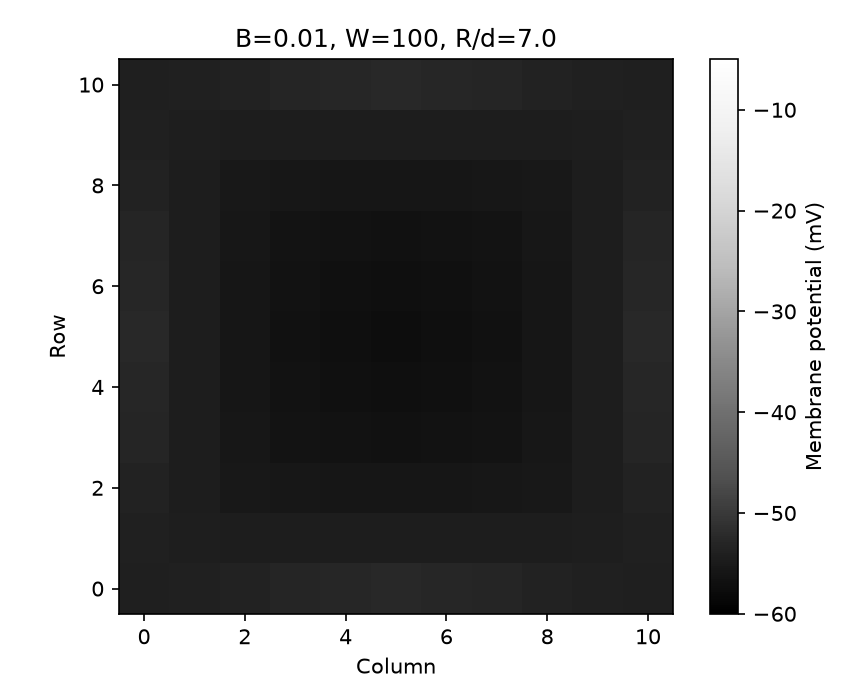
\includegraphics[width=\linewidth]{Screenshot 2026-10-02 215810} 
    \caption{W = 100, B = 0.01, R = 7*d} 
    \label{fig:sub-eq1} 
\end{subfigure} 
\hfill 
\begin{subfigure}[b]{0.32\textwidth} 
    \centering 
    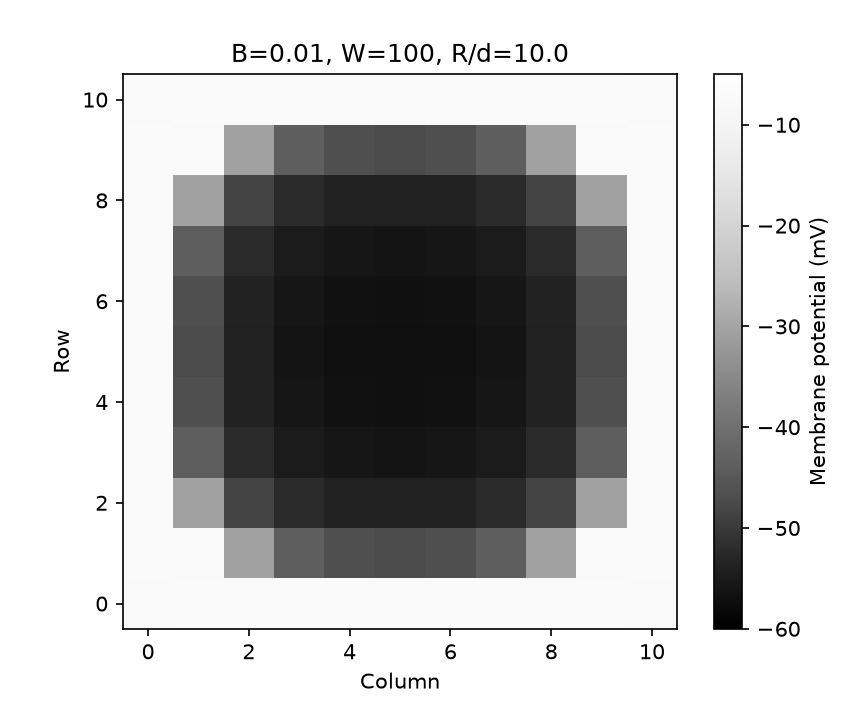
\includegraphics[width=\linewidth]{Screenshot 2026-10-02 220032} 
    \caption{W = 100, B = 0.01, R = 10*d} 
    \label{fig:sub-eq2} 
\end{subfigure} 
\hfill 
\begin{subfigure}[b]{0.32\textwidth} 
    \centering 
    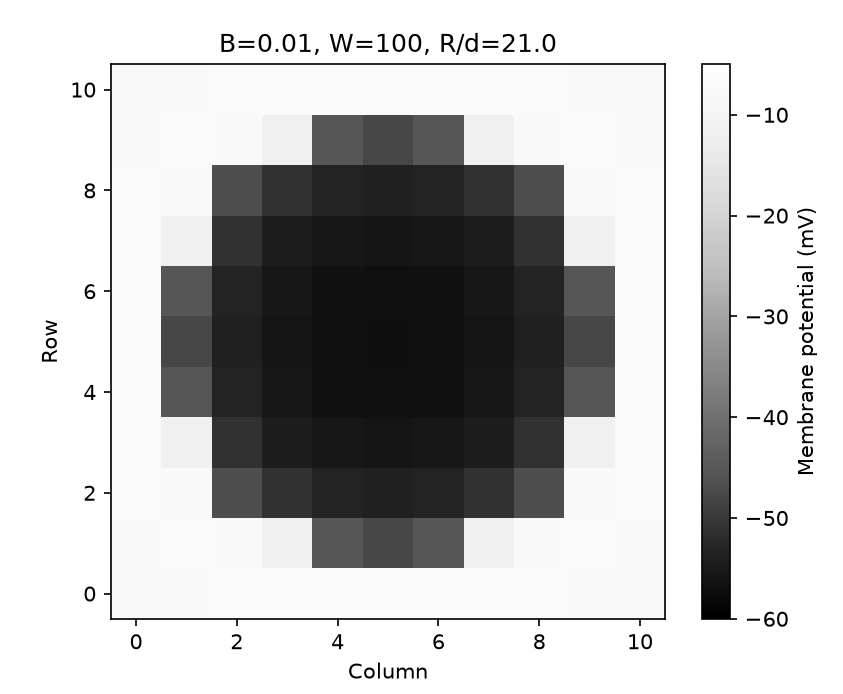
\includegraphics[width=\linewidth]{Screenshot 2026-10-02 220209} 
    \caption{W = 100, B = 0.01, R = 21*d.} 
    \label{fig:sub-eq3} 
\end{subfigure}

\vspace{2ex} % Adds vertical space between the two rows

% --- Second Row of Subfigures ---
\begin{subfigure}[b]{0.32\textwidth} 
    \centering 
    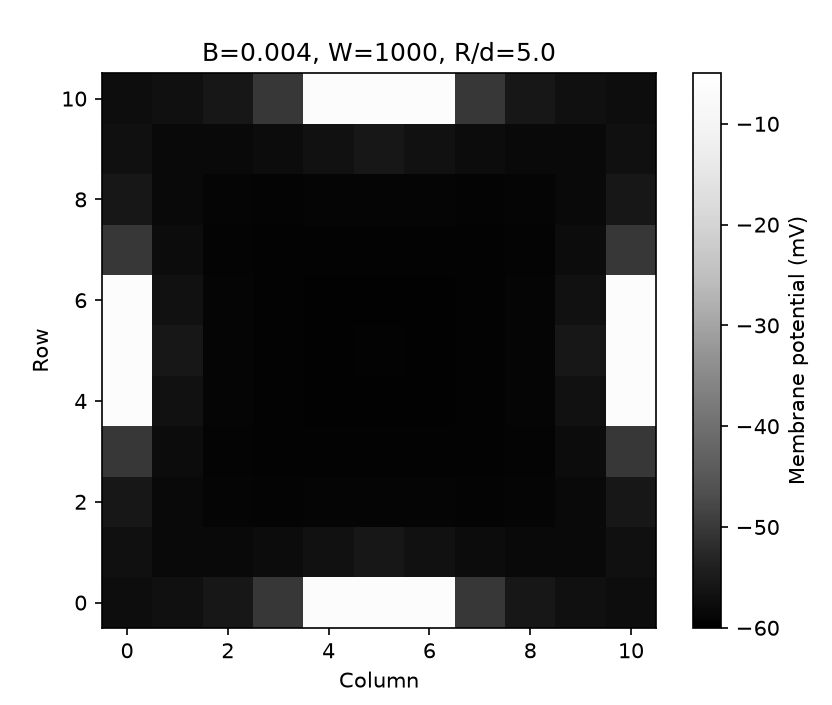
\includegraphics[width=\linewidth]{Screenshot 2026-10-02 221049} % Replace with your image path
    \caption{W = 1000, B = 0.004, R = 5*d.} 
    \label{fig:sub-eq4} 
\end{subfigure} 
\hfill 
\begin{subfigure}[b]{0.32\textwidth} 
    \centering 
    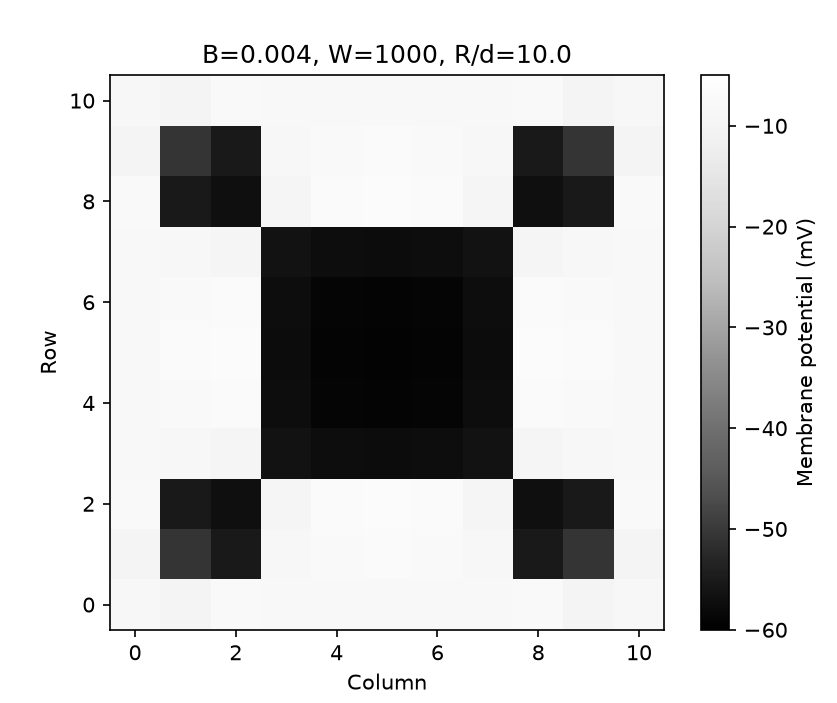
\includegraphics[width=\linewidth]{Screenshot 2026-10-02 221313} % Replace with your image path
    \caption{W = 1000, B = 0.004, R = 10*d.} 
    \label{fig:sub-eq5} 
\end{subfigure} 
\hfill 
\begin{subfigure}[b]{0.32\textwidth} 
    \centering 
    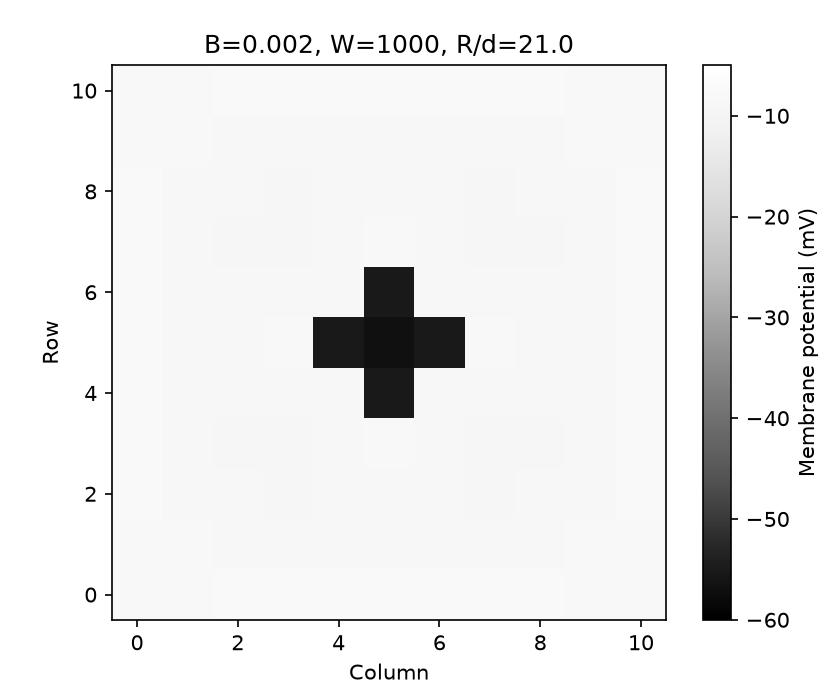
\includegraphics[width=\linewidth]{Screenshot 2026-10-02 221453} % Replace with your image path
    \caption{W = 1000, B = 0.002, R = 21*d.} 
    \label{fig:sub-eq6} 
\end{subfigure}
\caption{Spatiotemporal $V_{mem}$ patterns. Top row shows outcomes with weak field sensitivity (low W and high B), and the bottom row with strong field sensitivity (high W and low B). The columns represent different field action ranges $R$, from left to right, short, intermediate and long ranges. Plots are recorded for final state at $t = 5 s$ with 5001 output points. Shades represent cell $V_{mem}$ states, with darker representing hyperolarised and lighter representing depolarised cells respectively. } 
\label{fig:combined_screenshots} 
\end{figure}
\begin{flushleft}
The initial conditions for \textbf{Figure 4} simulations set all cells to $-55 mV$. It can be seen that the most heterogeneous spatial patterns of $V_{mem}$ occur for strong field sensitivity (high W and low B) and intermediate field action range, R. It is expected that this will correlate with the highest TSE complexity entropy as well (CHECK). \textbf{Figure 4 (a) -- (c)}, show increasing field action range with weak field sensitivity results in increasing the strength of the spatial pattern, comprising hyperpolarized center and depolarised peripheral cells. Strong field sensitivity in \textbf{(d) -- (f)} resulted in more complex $V_{mem}$ patterns, while this is maximized for intermediate field action range \textbf{(e)}, it is overridden for larger field action ranges \textbf{(f)} resulting in a simpler pattern resembling a more spatially defined version of \textbf{(c)}.
\hfill\break
\hfill\break
We now ran simulations on the $11 \times 11$ cell lattice, by sweeping across the parameters G, W, B, and R. 
\end{flushleft}

\end{document}